\part{Un corpus déjà structuré}

\clearpage
\thispagestyle{empty}
\cleardoublepage
\vspace*{\stretch{0.3}}
Le corpus sur lequel nous avons travaillé est un ensemble de fichiers XML-TEI. Ces derniers résultent d'une version numérisée des \odm{} réalisée et hébergée par le site \ia, elle-même issue du traitement des volumes physiques de l'Université de Toronto. Dans cette première partie, nous allons décrire ces différents états des \odm{} et commenter les opérations qui ont mené à leur structuration, tout en interrogeant les raisons ayant conduit le programme \timeus{} à les privilégier par rapport à d'autre version similaires.
\vspace*{\stretch{1.7}}

\chapter{Un corpus d'imprimés}

\section{Une publication sur une soixantaine d'années}

La publication des trois séries des \odm{} s'échelonne sur soixante-treize années (1857-1930). Elle n'est véritablement continue que sur trois périodes, de 1857 à 1862, puis de 1885 à 1913 et enfin de 1928 à 1930. L'interruption entre 1913 et 1928 est une conséquence de la première Guerre mondiale et des difficultés budgétaires auxquelles la \sess{} doit faire face après celle-ci. La première interruption, entre 1862 et 1885, est quant à elle due à un recalibrage des objectifs de la \sess, qui considère que \og continuer à recueillir des faits sans essayer d'en faire sortir aucune conclusion (...) c'eût été (...) une preuve d'impuissance et de stérilité \fg{}\footcite[p. I]{averts1t5}. Elle se concentre dès lors sur la parution de son \textit{Bulletin} jusqu'au début des années 1880, où \og le besoin de conclusions pratiques était amplement satisfait \fg{} et \og reprendre l'œuvre des monographies de familles \fg{} devenait possible\footcite[p. II]{averts1t5}.

Une tentative de reprise avait déjà été effectuée en 1875 où \og un premier fascicule composé de trois monographies \fg{} avait paru\footcite[p. III]{averts1t5}. Deux autres paraissent en 1883 et 1884, et les trois sont finalement rassemblés en 1885 dans le cinquième volume de la première série\footcite[p. III]{averts1t5}. Ce volume apparaît ainsi à bien des égards comme un moment charnière dans l'histoire de la publication des \odm. En effet, les monographies suivantes des deuxième (1887-1899) et troisième série (1904-1930) sont publiées sous forme de fascicules trimestriels qui sont ensuite reliés en volumes, là où les quatre premiers tomes étaient directement parus en volumes\footnote{\cite[p. 124]{lorry}.}. Des éléments de paratexte sont systématiquement fournis aux relieurs, notamment une page de titre, une introduction au volume, un index, des errata et une table des matières.

Le passage des volumes reliés aux fascicules trimestriels est acté par l'éditeur dans l'\textit{Avertissement} liminaire du premier fascicule de la deuxième série :

\begin{quote}
    \og La nouvelle série des \odm{} s'ouvre avec 
le présent fascicule. Le grand nombre des travaux soumis à la 
Société d'Économie sociale assure l'avenir et la régularité 
de la publication. \textit{Les monographies paraîtront désormais en 
fascicules trimestriels}\footnote{\cite[\og Avertissement \fg{}]{mono047a}. Nous soulignons.}. \fg{}
\end{quote}

Dans l'\textit{Avertissement} général de ce volume, édité en 1887 et placé immédiatement après la page de titre et le sommaire, le changement est à nouveau annoncé, mais également justifié :

\begin{quote}
    \og Quand la Société d'Économie sociale, en 1882, perdit celui qui 
avait réglé son rôle auprès de lui et après lui\footnote{Frédéric Le Play est mort le 5 avril 1882.}, elle trouva le cinquième tome des \odm{} arrêté au premier tiers de sa publication : elle acheva de le mettre au jour. Puis, voulant laisser bien distincts des travaux accomplis sous l'\oe{}il du maître, ceux dont il lui fallait dès lors prendre seule la responsabilité, \textit{elle commença en juillet 1885, sous le même titre, une nouvelle série de monographies de familles paraissant par fascicules trimestriels}\footnote{\cite[spec. p. II]{s2avert}. Nous soulignons.}. \fg{}
\end{quote}

\begin{figure}[t]
    \centering
    \begin{subfigure}[t]{0.4\textwidth}
     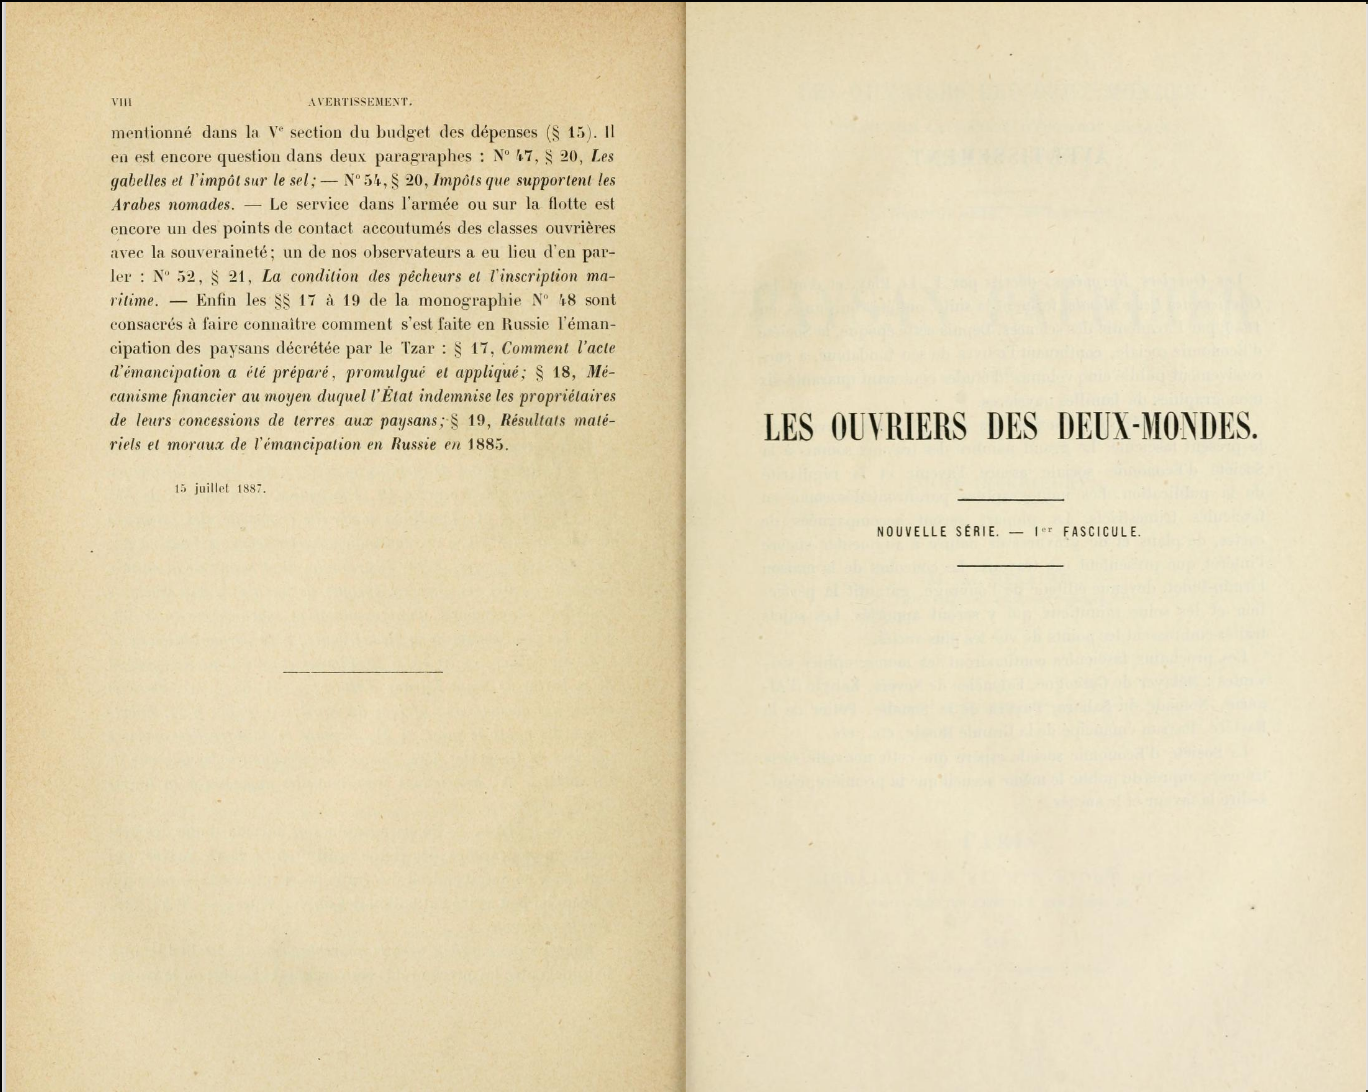
\includegraphics[width=1\linewidth]{img/odm47_ia_1.png}
     \caption{}
     \label{odm47ia1}
    \end{subfigure}
    \hspace{5pt}
    \begin{subfigure}[t]{0.4\textwidth}
     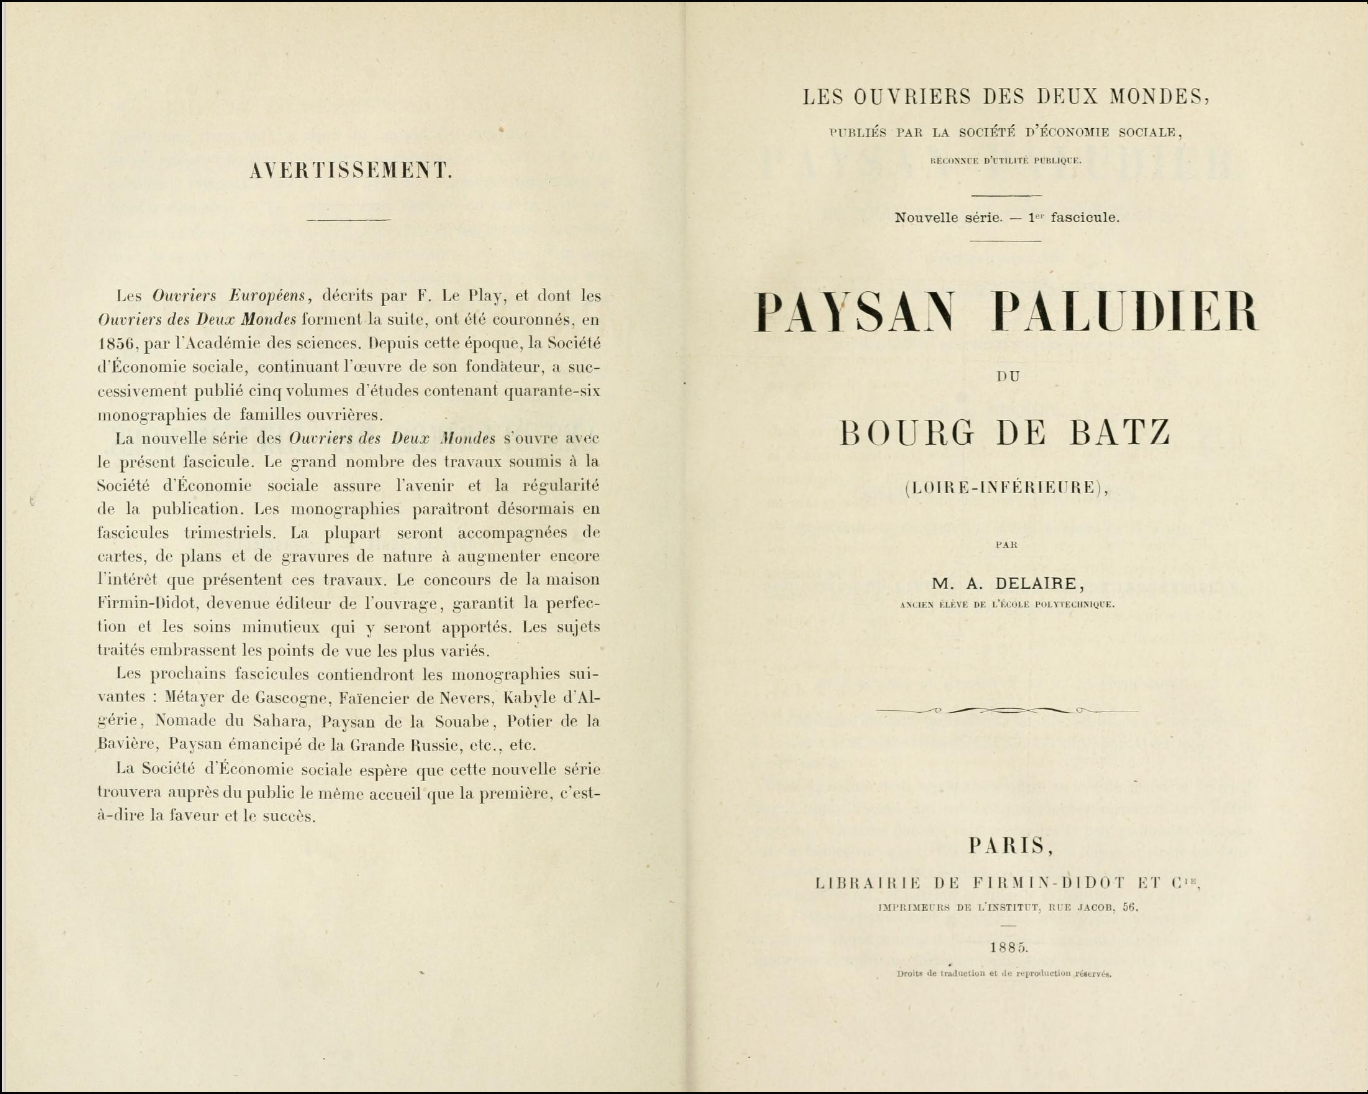
\includegraphics[width=1\linewidth]{img/odm47_ia_2.png}
     \caption{}
     \label{odm47ia2}
    \end{subfigure}
    \hspace{5pt}
    
    
    
    \begin{subfigure}[t]{0.4\textwidth}
     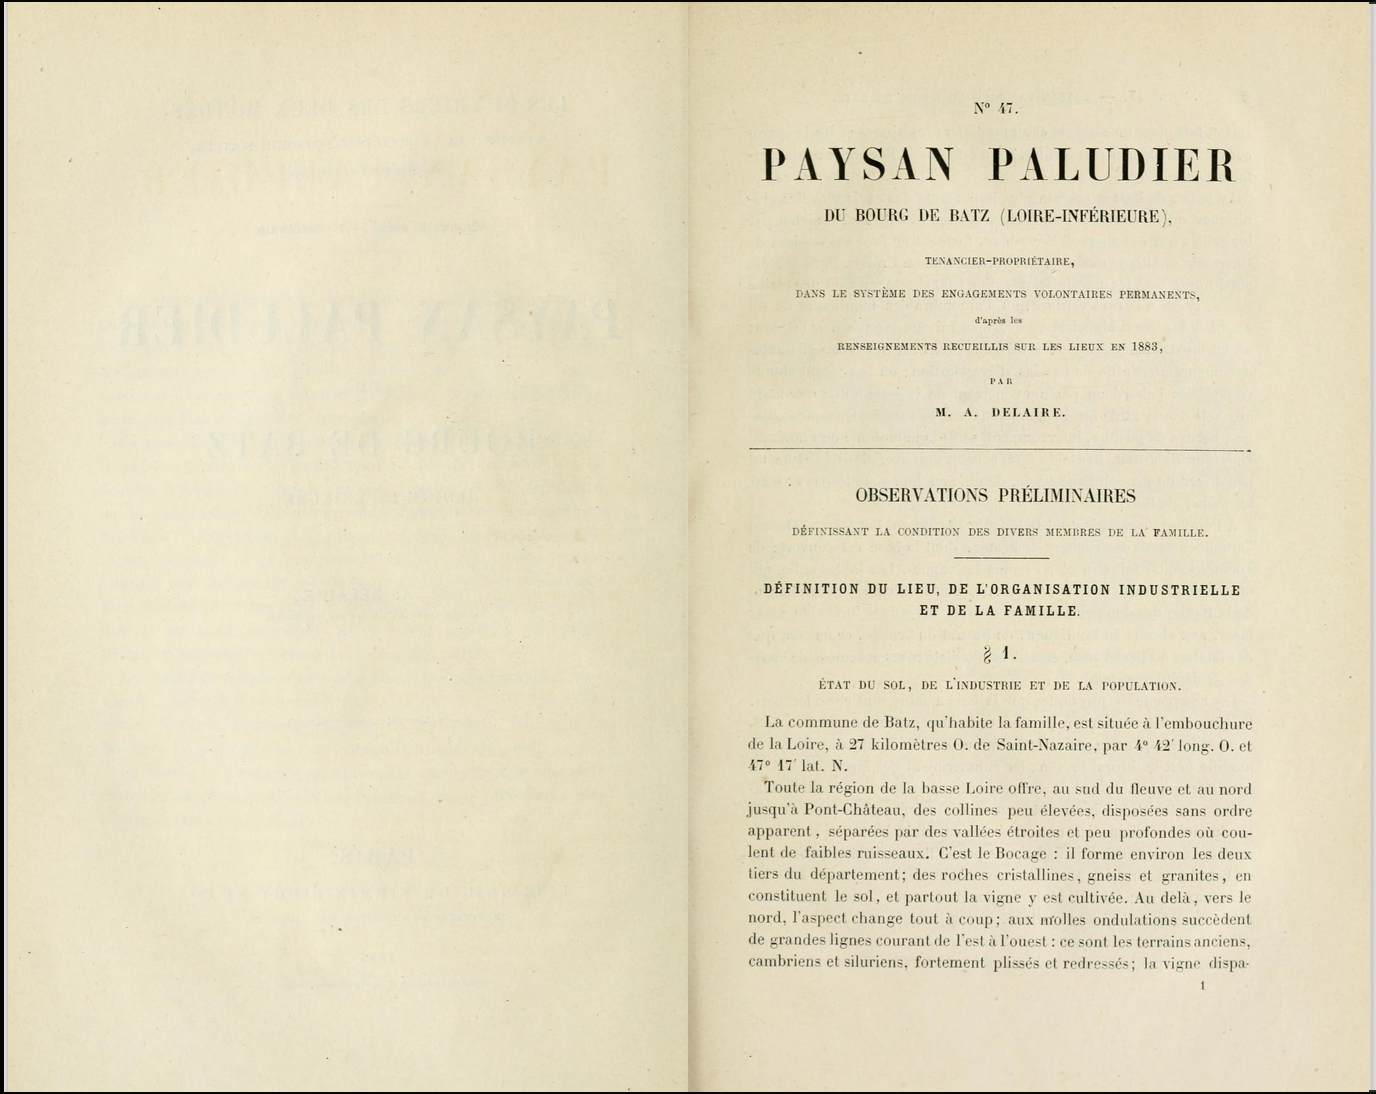
\includegraphics[width=1\linewidth]{img/odm47_ia_3.png}
     \caption{}
     \label{odm47ia3}
    \end{subfigure}
    \hspace{5pt}
    \begin{subfigure}[t]{0.4\textwidth}
     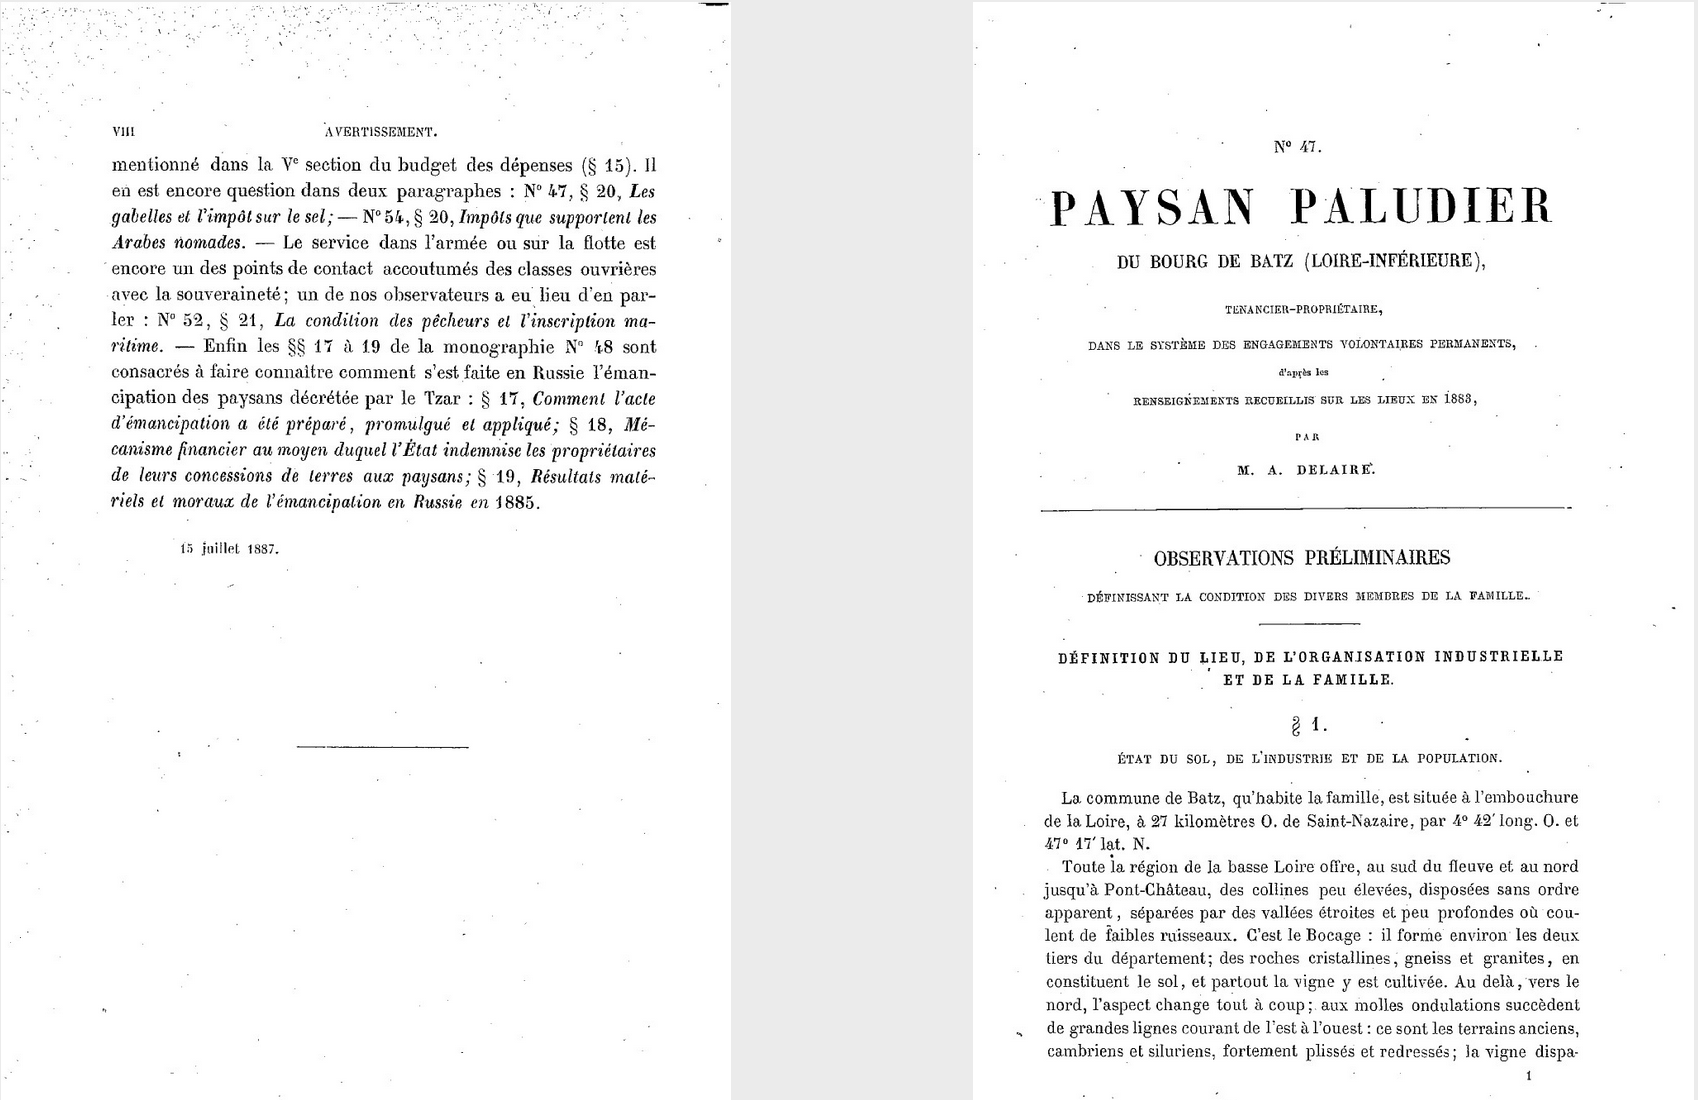
\includegraphics[width=1\linewidth]{img/odm47_bnf_1.png}
     \caption{}
     \label{odm47bnf}
    \end{subfigure}
    \caption{Comparaison des exemplaires de Toronto et de Paris. (a)~Toronto. Fin de l'\textit{Avertissement} général du volume et début du fascicule. (b)~Toronto. \textit{Avertissement} du fascicule et page de titre de la monographie. (c)~Toronto. Début de la monographie. (d)~Paris. Fin de l'\textit{Avertissement} général du volume et début de la monographie.}
    \label{odm47}
\end{figure}

Deux versions de ce même volume sont à notre disposition. L'une résulte de la numérisation de l'exemplaire déposé à la Bibliothèque nationale de France à Paris et conservé par le département Philosophie, histoire, sciences de l'homme\footnote{Consultable sur \textit{Gallica} : \url{https://gallica.bnf.fr/ark:/12148/bpt6k54465138} (consulté le \today).}, la seconde se trouve à la \textit{John P. Robarts Research Library} de l'Université de Toronto et a été numérisée par \ia\footnote{Consultable à cette adresse : \url{https://archive.org/details/s2lesouvriersdes01sociuoft} (consulté le \today).}.

Des différences de composition existent. Ainsi, l'exemplaire de Toronto (\fig{} \ref{odm47ia1}, \ref{odm47ia2}, \ref{odm47ia3}) comporte deux feuillets qui ne sont pas présents dans celui de Paris (\fig{} \ref{odm47bnf}). Le premier porte au recto le titre des \odm{} et au verso l'\textit{Avertissement} que nous avons cité ci-dessus en premier, le second est la page de titre du fascicule avec un verso vierge. Dans l'exemplaire de la Bibliothèque nationale, la première page de la monographie n° 47 suit la fin de l'\textit{Avertissement} général du volume.

Laisser aux propriétaires le soin de relier les fascicules pour composer le volume final revient à rompre l'unité codicologique de ce dernier, chaque nouvelle opération de reliure donnant naissance à un nouvel exemplaire. Les relieurs ont en effet pu choisir de conserver ou de ne pas conserver les pages propres aux fascicules, à l'instar des feuillets de l'exemplaire de Toronto. Il n'existe donc pas un modèle ayant autorité dans la composition des \odm{} --- en dépit du fait que les volumes de la Bibliothèque nationale de France, issus du dépôt légal, ont dû être versés par l'éditeur, \cad{} la Société internationale des études pratiques d'économie sociale.

Pour le projet \timeus{}, cela signifie que le corpus retenu pour le traitement informatisé et la publication finale ne sera qu'une version de l'\oe{}uvre que représente les \odm.

\section{La structure logique des monographies}

Un élément remarquable traverse la centaine de monographies des \odm{} : une même structure logique que les éditeurs ont tenté de maintenir tout au long de la publication.

Cette structure est l'incarnation de la méthodologie leplaysienne des monographies de familles. Le terme \textit{monographie}, \og emprunté à l'histoire naturelle et à la médecine \fg{}, qualifie au \textsc{xix}\ieme ~siècle une \og étude scientifique, minutieuse et détaillée, portant sur un objet ou un phénomène circonscrit \fg{}\footnote{\cite[p. 12]{savoye2}.}. La démarche monographique cherche à embrasser à travers l'observation directe des phénomènes inatteignables pour la démarche statistique, à laquelle elle s'oppose\footnote{Voir en particulier la charge de F. Le Play contre les statisticiens dans son introduction aux \textit{Ouvriers européens} de 1855 : \og La méthode des statisticiens n'est pas l'observation directe des faits ; c'est la compilation et l'interprétation plus ou moins plausible de faits recueillis à des points de vue fort différents, étrangers pour la plupart à l'intérêt scientifique. Malgré leur généralité apparente et leur séduisante régularité, les statistiques ont médiocrement contribué au progrès de la science sociale \fg{} : \cite[p.~11]{oe1855}.}.

Avant les \odm, Frédéric Le Play s'attelle aux \textit{Ouvriers européens}, recueil paru en 1855 et réédité en de 1877 à 1879, contenant trente-six (1\iere{}~éd.) puis cinquante-sept (2\ieme{}~éd.) monographies issues d'enquêtes menées entre 1833 et 1853\footnote{Inventaire complet dans \cite[p. 106-112]{lorry}.}. Les \odm{} se présentent comme une suite élargie à des espaces extra-européens de ce premier mouvement, dont ils reprennent la démarche, la structure et auquel ils font régulièrement référence par un système de renvoi. La structure logique des \odm{}, dont le premier volume est publié en 1855, est donc déjà présente dans \textit{Les Ouvriers européens}.

Elle procède d'une méthode d'observation que Le Play ne décrit qu'en 1862, au moment de la parution du quatrième volume des \odm{}. Le titre de cette méthodologie précise néanmoins qu'elle a déjà fait ses preuves pour les \textit{Ouvriers européens} : \textit{Instruction sur la méthode d'observation dite des monographies de familles, propre à l'ouvrage intitulé} Les ouvriers européens\footcite{instruction62}.

L'\textit{Instruction} est divisée en quatre parties suivies d'une cinquième faisant office de conclusion. Dans la première, Le Play circonscrit son champ d'observation à la famille ouvrière\footcite[I., \og Remarques préliminaires sur l'étude des faits sociaux et sur la méthode des monographies de familles \fg{}, p. 15-16]{instruction62}, érigée en \og clef de compréhension des organisations sociales \fg{}\footcite[p. 15]{savoye2}. La phase d'observation est ensuite divisée en étapes \footcite[II., \og Règles à suivre pour procéder à l'observation des faits sociaux \fg{}, p. 17-19]{instruction62}, savoir l'observation des faits, l'interrogatoire de l'ouvrier et celui des personnes tiers\footcite[p. 16]{savoye2}.

La troisième partie est celle où Le Play expose la structure logique qu'il utilise à partir de 1855 et que ses continuateurs reprennent jusqu'en 1930.
Elle est construite en miroir aux différentes phases de l'observation sur le terrain : à l'observation des faits répond la section des observations préliminaires, à l'interrogatoire de l'ouvrier celle des budgets et aux contacts avec les tiers celle des notes\footcite[III., \og Précis des faits à observer --- Établissement des budgets \fg{}, p. 20-31]{instruction62}. Le miroir est cependant légèrement déformant, afin de satisfaire au \og hiatus \fg{} propre à la démarche leplaysienne, entre les \og faits observés \fg{} et les \og faits décris \fg\footcite[p. 87]{baciocchi2}. L'observation est en effet \og contrainte par l'évidence des choses \fg{} là où la description, \og parce qu'elle suppose de désigner précisément ce qu'on évoque, repose sur un calibrage sémantique \fg{}\footcite[p. 87-88]{baciocchi2}. La structure logique des monographies de familles n'est donc pas qu'un simple plan de rédaction, elle procède d'une démarche intellectuelle réglée par Le Play et doit être appliquée pour garantir la validité de la démonstration.

Cette structure (\ann{} \ref{structure}) possède trois niveaux de titre : les parties~(A, B, C), les sections~(I, II, etc.) et les paragraphes~(§1, §2, etc.). Le dernier niveau est toujours atteint dans la partie~B (\textit{Observations préliminaires}), mais très rarement dans la partie~C (\textit{Notes}).

\begin{figure}[h]
    \centering
    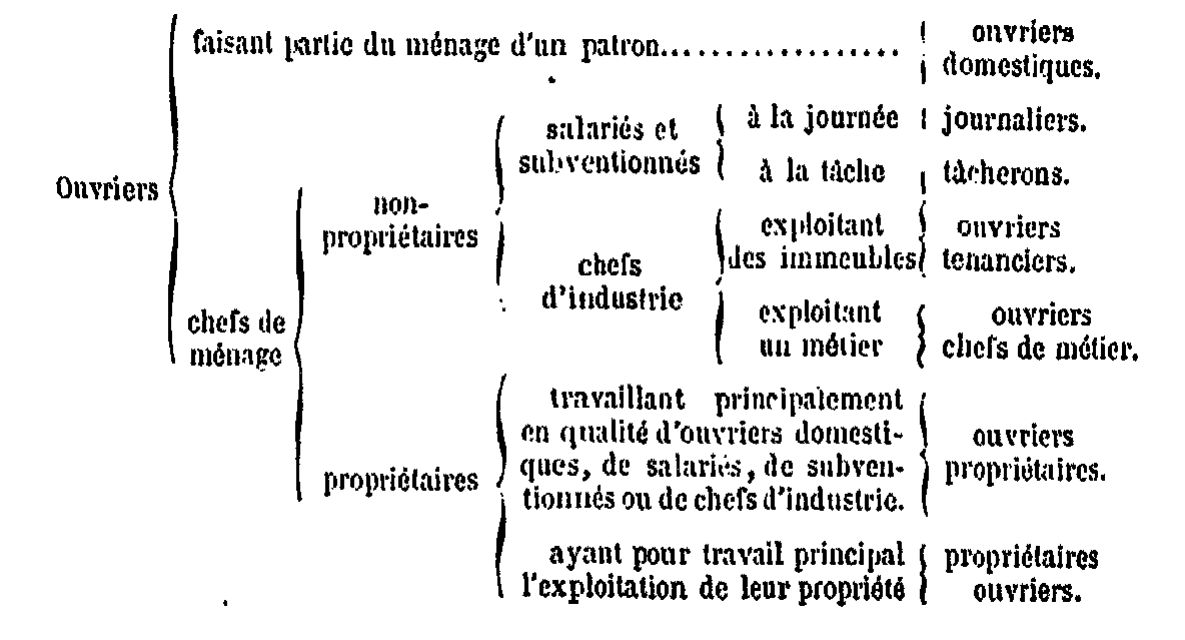
\includegraphics{img/tabl_titres.jpg}
    \caption{\og Tableau des sept situations principales que les ouvriers peuvent occuper successivement dans les quatre systèmes sociaux pour s'élever des rangs inférieurs de la hiérarchie industrielle à la condition de propriétaires ou de chefs d'industrie. \fg{}, permettant de construire le titre d'une monographie de famille (capture d'écran de \textit{Gallica}).}
    \label{tabletitre}
\end{figure}

La première partie~(A) est la page de titre. Le titre de la monographie est présenté comme le \og résumé \fg{} de celle-ci, et doit pour cela contenir quatre éléments imprescriptibles : \og 1° la profession de l'ouvrier, 2° la population dont il fait partie, 3° la nature des engagements qu'il contracte pour se procurer des moyens de travail, 4° la situation qu'il occupe dans l'organisation sociale caractérisée par cet engagement \fg{}\footcite[p. 20]{instruction62}. Ainsi, en dépit dut fait que Le Play ne considère pas explicitement la page de titre comme une composante de sa structure, l'importance qu'il donne au titre en lui-même a conduit le projet \timeus{} à l'interpréter comme telle. Un tableau pour construire ce titre est d'ailleurs mis à la disposition des monographes (\fig{} \ref{tabletitre}\footcite[p. 21 .]{instruction62}).

\section[Continuité, discontinuité et erreurs d'impression]{Continuité, discontinuité et erreurs d'impression dans la structure logique}

En dépit de son aspect monolithique, la structure logique des monographies de familles subit plusieurs ajustements au cours de la publication. Certains, uniquement de circonstance, sont des évènements mineurs, là où d'autres sont des changements significatifs adoptés pour la suite de la publication.

La monographie n° 85 représente ainsi un tournant dans la numérotation des titres de paragraphe, sans pour autant changer leurs libellés (\ann{} \ref{structure}). En effet, la numérotation cardinale est étendue au dernier paragraphe des budgets (\textit{Comptes annexés aux budgets}) et remplace la numérotation alphabétique utilisée auparavant dans la partie \textit{Notes}.

Pourquoi cette uniformisation intervient-elle à partir de cette monographie, en plein milieu du cinquième volume ? Nous avons vu plus haut que ce volume représentait un tournant dans la publication des \odm, notamment en raison de la mort de Frédéric Le Play qui intervient avant qu'il ne soit achevé. Il est possible le départ du fondateur de la série ait permis d'opérer des changements dans la structure qu'il avait créée, ou bien que ce soit Le Play lui-même qui ait voulu ces changements. Quoi qu'il en soit, il y a une volonté claire de renforcer la solidité de la démonstration en rassemblant ses différents paragraphes en un seul bloc par le biais d'une numérotation cardinale continue. Le nombre moyen de paragraphes est de 21 ; la monographie la plus longue, composée de trente-cinq paragraphes, étant la n° 64, intitulée \textit{Paysans corses en communauté, porchers-bergers des montagnes de Bastelica}\footcite{mono064a}.

\chapter{Des numérisations multiples}

Début du deuxième chapitre

\chapter{Un encodage automatique}

Début du troisième chapitre